\chapter[Introdução]{Introdução}

\section{Contexto}

O monitoramento da qualidade das águas é ação principal para a identificação, análise e prevenção de problemas, recuperação e melhoria da condição ambiental do planeta. Este é o início das transformações de conduta do seres humanos em relação aos rios, lagos e mares pois explicita ainda mais que estes precisam de uma maior atenção e cuidado. 
 
Sem água não haveria vida. Ela é de extrema importância para a vida de todos os seres vivos. Embora este recurso esteja presente em 70\% da superfície terrestre, só 4\% dela é referente a água doce, ou seja, água própria para consumo. Fazendo uma análise de que o planeta possui 7 milhões de habitantes e esse número vem crescendo, monitorar e cuidar dessa água é de suma importância e se transforma no desafio do milênio. 

Principais funções que tornam a água importante:

\begin{itemize}
    \item Funcionamento e manutenção do corpo humano.
    \item Produção de alimentos para os seres humanos (Pecuária e Agricultura). 

    \item Uso da água na produção industrial (bens materiais, medicamentos, alimentos industrializados, etc.).

    \item Geração de energia nas usinas hidrelétricas.

    \item A evaporação da água doce das principais fontes hídricas (rios, lagos, açudes e represas) são importantes na formação de chuvas e da umidade do ar.


\end{itemize}


A água de qualidade também é essencial para os nossos ecossistemas. As plantas e animais reagem a mudanças em seu ambiente causadas por mudanças na qualidade da água química e perturbação física de seu habitat. Alterações na composição de espécies de grupos de organismos como fitoplâncton, algas, macrófitas, animais de fundo e peixes podem ser causadas por mudanças no clima (AErtebjerg, G., Andersen, J.H. e Hansen ,2003). 

Diante de todos os pontos levantados, o mundo busca soluções para a controlar e monitorar este recurso primordial a vida. Logo houveram projetos de barcos autônomos que coletam dados relativos a água. Este tipo de navegação normalmente é controlado por uma pessoa em terra através de um computador ou dispositivo portátil. Neste seguimento foi criado o barco autônomo, movido por energia solar, pela empresa Holos Brasil, que está situada no Rio de Janeiro. 

Este barco pode levar instrumentos para vários tipos de missão, tais como coleta de dados meteorológicos, oceanográficos ou fluviais (profundidade, traçado da topografia do leito) e para o estudo da vida aquática. 

 \begin{figure} [!htp]
	\centering
	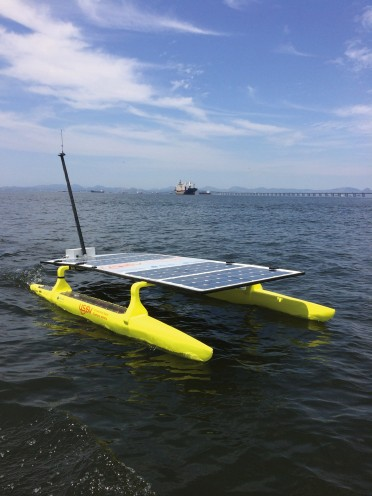
\includegraphics[scale=0.5]{figuras/barcoINTRODUCAO}
	\caption{Barco Autônomo Holos Brasil}
	\label{barcoINTRODUCAO}
\end{figure}

Entretanto, apesar de ter alcance elevado, ser bastante robusto e coletar diversas informações que não são referentes a qualidade da água e teve um custo muito alto, aproximadamente 300 mil reais. O que é inviável para grande parte dos projetos e pesquisas a serem desenvolvidas.


\section{Problema}

A declaração do problema e da visão deixa explícita a necessidade do negócio, identifica as principais partes interessadas e descreve brevemente o impacto positivo, que ao atender a necessidade do negócio, a mesma terá sobre as partes interessadas (Guia BABOK, 2011).

Dessa maneira, segue a declaração do problema ao qual o RoBoat busca resolver:

\begin{table}[h]
	\centering
	\label{tab01}	
	\begin{tabular}{ccc}
		\toprule
		\textbf{O problema de} & \textbf{Medir qualidade da água em determinados locais} \\
		\midrule
		Afeta & A população em geral         \\
		Impacto & Falta de informações sobre a qualidade da água.            \\
		Consequências &  Falta de ações para melhoria dela da água.\\
		Solução & Um barco autônomo de medição de água, com custo moderado.               \\
		\bottomrule
	\end{tabular}	
	\caption{Declaração do problema ao qual o RoBoat busca resolver}
\end{table}


\section{Justificativa}



O intuito do desenvolvimento do projeto é promover a interação entre as Engenharias de forma colaborativa, visando, ampliar o conhecimento dos alunos de cada um delas, de forma que haja uma de aprendizado multidisciplinar e que o conhecimento seja recíproco, funcional e operacional. 
O contexto a ser desenvolvido foi a criação de um Barco autônomo (RoBoat) que coleta água e dados da água de lagos, rios e reservatórios. Isso foi percebido, levando-se em consideração a importância da água aos seres vivos e explicitando a necessidade do monitoramento, controle e posteriormente, ações de prevenção e melhoramento das águas. 

Essa necessidade traz consigo outras, como a da coleta de informações da água em pontos onde há grande dificuldade das pessoas alcançarem sem que haja o aparato de uma embarcação comum, além da necessidade, de uma alternativa aos barcos autônomos que se encontram no mercado, que normalmente ou não coletam água, ou tem seus custos bastante elevados. Uma solução como essa, serviria como auxílio para pesquisas e estudos, o que beneficiaria toda a população através de possíveis atitudes que venham a ser tomadas a partir da utilização do RoBoat.


\section{Objetivos}

Objetivo Geral

Este  projeto  tem  por  objetivo  geral  a  construção  de  um  barco ao qual a aplicação será analisar informações da água de forma autônoma, além de coletar três amostras, em determinados locais previamente programados.

Objetivos por áreas:

1- Definir, projetar e construir a estrutura do Barco;

2- Definir, projetar e implementar a parte de alimentação e controle de motores;

3- Definir, projetar e construir o monitoramento e controle;

4- Definir, projetar e construir o software, tanto interface para usuário quanto comunicação remota e automação do RoBoat;

5- Integrar todos os módulos que compõem o RoBoat.


